\documentclass[11pt,a4paper]{article}
\usepackage{tikz}
\usetikzlibrary{arrows.meta,positioning}
\usepackage{tabularx}
\usepackage{amsmath,amssymb,amsthm}
\usepackage{geometry}
\geometry{margin=1in}
\usepackage{hyperref}
\usepackage{graphicx}
\usepackage{setspace}
\onehalfspacing

\title{\textbf{Paper A-07: Earth Biodiversity:\\ A Constraint-Driven Flux Dynamics (CDFD) Perspective}}
\author{Steve Bico Mujjabi, MD\\
\small Independent Researcher\\
\small Founder, Vura Labs\\
\small Kampala, Uganda\\
\small ORCID: 0009-0001-0556-5516}
\date{May 2026}

\begin{document}
\maketitle


\begin{abstract}
This paper develops a falsifiable CDFD/AFL model of Earth Biodiversity. It maps colonization, energy supply, disturbance, and environmental change to driving flux $\Phi$, habitat area, fragmentation, resource limits, and interaction structure to active constraint $C$, functional redundancy, dispersal, refugia, and adaptation to responsiveness $S$, and extinction debt, genetic erosion, invasion, and disturbance history to structural memory $M_s$. The target outcome is persistence, turnover, function, and extinction risk, tested against species inventories, occupancy time series, trait data, genetics, and remote sensing. The paper treats universality as a shared model architecture rather than an assertion that unlike systems have the same material mechanism. It states the negative result that would make the mapping unnecessary and places the domain claim inside the cumulative CDFD programme and its reproducible runtime boundary.
\end{abstract}

\section*{Symbol Conventions}

\noindent\textbf{CDFD/AFL Part IV symbol convention.}
\begin{center}
{\small
\begin{tabular}{p{0.15\linewidth}p{0.34\linewidth}p{0.41\linewidth}}
\hline
Symbol & Part IV meaning & Cross-domain reading \\
\hline
$\Phi$ & Driving flux or throughput & Energy, matter, signal, capital, information, traffic, force, or biological load entering a system \\
$C$ & Active constraint or capacity burden & Bottleneck, resistance, boundary, scarcity, toxicity, regulation, topology, latency, or load-bearing limit \\
$S$ & Responsiveness or adaptive surface & The system's ability to reconfigure, buffer, route, repair, learn, or preserve function under changing load \\
$M_s$ & Structural memory & Stored damage, hysteresis, inherited topology, institutional memory, trained weights, ecological legacy, or retained state \\
$\Psi_s$ & Adaptive operating ratio $(\Phi/C)\cdot S\cdot M_s$ & Local bookkeeping gauge for constrained operation, overload, recovery, or regime change; not a universal constant \\
$\Lambda$ & Life Number or capstone surplus ratio where explicitly defined & Reserved for Part II-derived life-number notation or synthesis-level surplus measures, never an undefined decoration \\
\hline
\end{tabular}
}
\end{center}

\noindent\textbf{Greek-symbol convention.}
\begin{center}
{\small
\begin{tabular}{p{0.15\linewidth}p{0.34\linewidth}p{0.41\linewidth}}
\hline
Symbol & Local role & Interpretation rule \\
\hline
$\alpha$ & Accumulation or reinforcement coefficient & Sets how fast a pathway, constraint, habit, cascade, or retained structure grows under load \\
$\beta$ & Relaxation, decay, clearance, or washout coefficient & Sets loss, recovery, damping, forgetting, degradation, or return toward baseline \\
$\gamma$ & Coupling, diffusion, redistribution, or transfer coefficient & Sets spread across nodes, layers, tissues, markets, infrastructures, media, or physical phases \\
$\delta,\epsilon$ & Perturbation, tolerance, small offset, or numerical guard & Used only as local thresholds, stability margins, measurement tolerances, or stress increments \\
$\eta,\lambda,\mu,\nu$ & Efficiency, rate, baseline, intensity, or frequency terms & Meaning is fixed by the equation, subscript, and domain-specific proxy in the paragraph where the term appears \\
$\rho,\sigma,\tau,\phi$ & Density/correlation, variability/noise, time-scale, phase, or field terms & Local coefficients only; subscripts bind them to the named pathway, domain, or experiment \\
$\Omega,\Lambda$ & Domain/state space; Life Number where defined & $\Omega$ names a modeled state space; $\Lambda$ carries life-number or synthesis notation only when the paper defines it \\
\hline
\end{tabular}
}
\end{center}

\section{Series Context}

Part I sets the flow--constraint language used here \cite{MujjabiPartI2026}. Part II develops the Life Number and the origins-of-life use of the same notation \cite{MujjabiPartII2026}. Part III applies AFL to biology and medicine \cite{MujjabiPartIII2026}. Part IV \cite{MujjabiPartIV2026}, DOI \url{https://doi.org/10.5281/zenodo.20395901}, is the cross-domain stress test: it asks where the notation clarifies measurement, and where it becomes only a metaphor.

\section{Introduction}

\subsection{The Mujjabi Universal Capacity Law}
Building directly upon the Fundamental Physics (Part I) \cite{MujjabiPartI2026}, the \textbf{Mujjabi Universal Capacity Law} proposes that across all scales---from black hole event horizons to global financial markets and power grids---driving high flux ($\Phi$) against a rigid topological constraint ($C$) can drive system saturation. When $\Phi/C$ approaches critical thresholds, the system does not scale linearly; it undergoes a topological phase transition.

\subsection{The Mujjabi Universal Memory Law}
The \textbf{Mujjabi Universal Memory Law} frames persistent systemic collapse. When a complex network fails to clear its structural memory ($M_s$) and its relaxation parameter decays ($\tau_{relax} \to \infty$), temporary stressors become permanent rigidities. This is the proposed CDFD mechanism behind ecological death, economic depressions, and infrastructural gridlock.

A rainforest and a monoculture cornfield may receive a comparable solar energy flux, yet their thermodynamic stability is vastly different. A minor drought will destroy the cornfield, while the rainforest barely registers the perturbation.

In CDFD, this resilience is not magic; it is pure topological elasticity. Biodiversity is the physical manifestation of an ecosystem's capacity to bend its constraints to absorb incoming flux.

\section{Biodiversity as Responsiveness ($S$)}
We govern the resilience of an ecosystem using the Universal Adaptive Ratio:
\begin{equation}
    \Psi_s = \left( \frac{\Phi}{C} \right) \cdot S \cdot M_s
\end{equation}

In an ecological context:
\begin{itemize}
    \item \textbf{Flux ($\Phi$)}: The total energetic and material throughput of the environment (sunlight, water, carbon).
    \item \textbf{Constraint ($C$)}: Environmental friction, such as temperature extremes, pathogens, or physical barriers.
    \item \textbf{Responsiveness ($S$)}: \textbf{Biodiversity}. The sheer number of different genetic and phenotypic pathways available to route energy. If one species fails, another immediately fills the niche, ensuring the total throughput $\Phi$ is maintained.
    \item \textbf{Memory ($M_s$)}: Ecological specialization. As environments remain stable for millions of years, species over-specialize to maximize efficiency, heavily locking the system into specific inter-dependencies.
\end{itemize}

\subsection{Monocultures and the Mathematics of Fragility}
In a highly diverse ecosystem, $S$ is large. If a constraint $C$ spikes (e.g., a new disease), the high $S$ ensures $\Psi_s$ remains stable near $1$.

In human-engineered monocultures (e.g., a vast plantation of genetically identical bananas), $S$ is artificially forced to a near-zero minimum. To keep the system producing ($\Psi_s \approx 1$), humans must artificially force the environmental constraints to zero ($C \to 0$) using massive applications of pesticides and fertilizers.

This state is a thermodynamic house of cards. The moment human intervention ceases and a natural constraint reappears ($C$ spikes), the denominator overwhelms the equation. Because $S$ is fundamentally broken, the system instantly collapses into a $\Psi_s \ll 1$ state of total necrosis.



\section{Measurement Layer}

The first job in any domain is to choose proxies before drawing conclusions. $\Phi$ may be a rate of material, energy, information, capital, or signal flow. $C$ is the bottleneck that slows or redirects that flow. $S$ measures the system's ability to reconfigure under stress, and $M_s$ records the past load that still changes present behavior. A useful application gives those four terms observable definitions, a time scale, and a failure condition. If a standard domain model explains the same data more cleanly, the CDFD/AFL mapping should give way.

\subsection{Current Runtime Diagnostic: Universal Network Cascade}
The release-local discovery script keeps this paper tied to the current CDFD Runtime \cite{CDFDRuntime2026}, including RK4 field updates, surface dynamics, structural-memory diffusion, and a finite-value audit. In the 2026-06-04 runtime pass, the localized hub-drive stress test ended with hub $\Psi_s=5.21$, peak network $\Psi_s=5.21$, 21 nodes above $\Psi_s>1.5$, and 37 maximum memory-locked nodes. I treat those numbers as a runtime sanity check and as a target for later domain measurement, not as a substitute for field data.


% BEGIN PART IV MAJOR UNIVERSAL UPGRADE
\section{Major Universal Upgrade: Mechanism, Scale, and Tests}

\subsection{Observable Translation}

The paper-specific translation begins with an observable chain rather than a
verbal analogy. For Earth Biodiversity, the proposed drive is colonization, energy supply, disturbance, and environmental change.
The active limitation is habitat area, fragmentation, resource limits, and interaction structure. Responsiveness is carried by
functional redundancy, dispersal, refugia, and adaptation, while retained state is represented by
extinction debt, genetic erosion, invasion, and disturbance history. The outcome to explain is persistence, turnover, function, and extinction risk.

\begin{table}[htbp]
\centering
\small
\caption{Operational CDFD/AFL map for Paper A-07.}
\begin{tabularx}{\textwidth}{|l|X|X|}
\hline
\textbf{Term} & \textbf{Paper-specific observable meaning} & \textbf{Measurement question} \\
\hline
$\Phi$ & colonization, energy supply, disturbance, and environmental change & What rate, load, gradient, or demand enters the focal system? \\
\hline
$C$ & habitat area, fragmentation, resource limits, and interaction structure & Which measured bottleneck limits transfer, function, or recovery? \\
\hline
$S$ & functional redundancy, dispersal, refugia, and adaptation & Which process changes effective capacity or reroutes the load? \\
\hline
$M_s$ & extinction debt, genetic erosion, invasion, and disturbance history & Which retained state makes equal present loads produce different futures? \\
\hline
$Y$ & persistence, turnover, function, and extinction risk & Which outcome is predicted out of sample, with uncertainty? \\
\hline
\end{tabularx}
\end{table}

\begin{figure}[htbp]
\centering
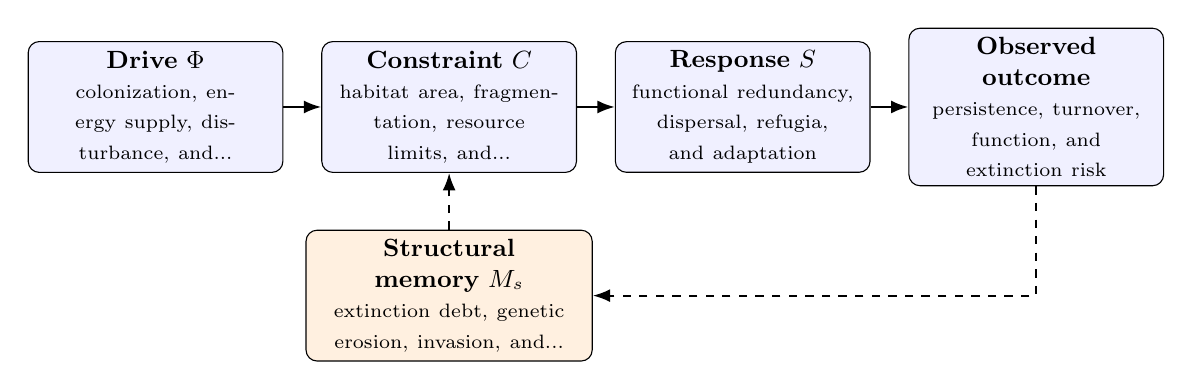
\begin{tikzpicture}[
    node distance=0.48cm,
    every node/.style={font=\small},
    box/.style={draw, rounded corners, align=center, minimum height=1.45cm, text width=3.0cm, fill=blue!6},
    memory/.style={draw, rounded corners, align=center, minimum height=1.25cm, text width=3.4cm, fill=orange!12},
    flow/.style={-{Latex[length=2.2mm]}, thick},
    feedback/.style={-{Latex[length=2.2mm]}, thick, dashed}
]
\node[box] (drive) {\textbf{Drive $\Phi$}\\\scriptsize colonization, energy supply, disturbance, and...};
\node[box, right=of drive] (constraint) {\textbf{Constraint $C$}\\\scriptsize habitat area, fragmentation, resource limits, and...};
\node[box, right=of constraint] (response) {\textbf{Response $S$}\\\scriptsize functional redundancy, dispersal, refugia, and adaptation};
\node[box, right=of response] (outcome) {\textbf{Observed outcome}\\\scriptsize persistence, turnover, function, and extinction risk};
\node[memory, below=0.72cm of constraint] (memory) {\textbf{Structural memory $M_s$}\\\scriptsize extinction debt, genetic erosion, invasion, and...};
\draw[flow] (drive) -- (constraint);
\draw[flow] (constraint) -- (response);
\draw[flow] (response) -- (outcome);
\draw[feedback] (outcome.south) |- (memory.east);
\draw[feedback] (memory.north) -- (constraint.south);
\end{tikzpicture}
\caption{Paper A-07 observable CDFD/AFL architecture for Earth Biodiversity. Solid arrows give the proposed forward chain; dashed arrows make history-dependent feedback explicit.}
\label{fig:a07-architecture}
\end{figure}

\subsection{Minimal Coupled Model}

A paper-level model must separate throughput, constraint accumulation, response,
and history. One deliberately minimal form is
\begin{align}
Y(t) &= \frac{\Phi(t)S(t)}{\epsilon + C(t)}, \\
\frac{dC}{dt} &= \alpha \Phi(t) - \beta S(t)C(t) + \gamma \mathcal{L}C(t), \\
\frac{dM_s}{dt} &= \eta C(t) - \mu M_s(t), \\
\Psi_s(t) &= \frac{\widehat{\Phi}(t)}{\epsilon+\widehat{C}(t)}\,
             \widehat{S}(t)\,[1+\omega\widehat{M_s}(t)] .
\end{align}
Here $Y$ is the measured output, $\epsilon>0$ prevents a singular denominator,
$\mathcal{L}$ is a spatial or network coupling operator, and hats denote
explicitly normalized variables. The sign and magnitude of $\omega$ must be
estimated: memory can preserve useful organization or amplify damage. No fixed
threshold is universal before the variables, normalization, and observation
scale are declared.

For this paper, the hypothesized causal sequence is specific. A change in
colonization, energy supply, disturbance, and environmental change arrives faster than functional redundancy, dispersal, refugia, and adaptation can compensate.
This raises or redistributes habitat area, fragmentation, resource limits, and interaction structure. If the load persists,
the retained state encoded by extinction debt, genetic erosion, invasion, and disturbance history changes the next response, so a later event of equal
magnitude can produce a different trajectory in persistence, turnover, function, and extinction risk. The
scientific task is to estimate that sequence against the best ordinary model of
the domain, not merely to redescribe the outcome after it occurs.

\subsection{Cross-Scale Universality Without Mechanistic Erasure}

For the Earth systems family, the universal comparison is between coupled transport, finite environmental capacity, buffering, and retained landscape or ecosystem state. Universality here cannot erase conservation laws, geometry, or scale; it must expose where those domain equations create comparable overload and recovery structures. \cite{Holling1973,Turing1952,BakTangWiesenfeld1987}
The CDFD programme is cumulative: Part I supplies the flow--constraint
foundation \cite{MujjabiPartI2026}; Part II asks when maintained throughput
supports persistent organized states \cite{MujjabiPartII2026}; Part III
develops adaptive limitation and biological memory \cite{MujjabiPartIII2026};
and Part IV \cite{MujjabiPartIV2026} tests how much of that architecture
survives translation. The CDFD Runtime \cite{CDFDRuntime2026} supplies a
reproducible numerical stress surface, but it does not substitute for the
domain evidence named here.

The required scale declaration for this paper is generations to millennia; populations to biomes. At short
scales, the key question is whether the incoming drive is transmitted,
buffered, or diverted. At intermediate scales, response changes effective
capacity and network exposure. At long scales, retained structure can alter the
state space itself. A result is genuinely cross-scale only when the aggregation
rule is stated and the same conclusion is not an artifact of averaging.

\subsection{Evidence Ladder and Discriminating Tests}

\begin{table}[htbp]
\centering
\small
\caption{Evidence ladder for Paper A-07. Each rung can fail independently.}
\begin{tabularx}{\textwidth}{|p{0.17\textwidth}|X|X|}
\hline
\textbf{Test} & \textbf{Design} & \textbf{Discriminating result} \\
\hline
Proxy audit & Measure species inventories, occupancy time series, trait data, genetics, and remote sensing and preregister how each record maps to $\Phi$, $C$, $S$, $M_s$, and $Y$. & The mapping fails if proxies are non-identifiable, circular, or change meaning across cases. \\
\hline
Load ramp & Apply or observe fragmentation followed by reconnection or habitat restoration while estimating the dominant constraint and response time. & A threshold claim requires a reproducible nonlinear change and uncertainty bounds, not a visually chosen breakpoint. \\
\hline
Recovery and memory & Match present load across units with different histories, then compare recovery paths. & The memory claim requires history-dependent divergence after current conditions are controlled. \\
\hline
Model comparison & Compare the baseline domain model with and without the CDFD/AFL state variables using held-out data. & The paper's stated falsifier is: prior fragmentation history does not alter recovery after present habitat is matched. \\
\hline
\end{tabularx}
\end{table}

The strongest practical design combines a prospective perturbation with a
recovery window. The load-ramp phase estimates where constraint begins to rise
faster than output. The recovery phase estimates $\beta$ and $\mu$, separating
fast relaxation from persistent memory. A topology or coupling intervention
then asks whether rerouting changes the cascade as predicted. Null results are
informative because they identify domains in which the universal notation adds
no measurable value.

\subsection{Research Programme and Boundary Conditions}

The immediate research programme has four steps. First, construct a documented
dataset from species inventories, occupancy time series, trait data, genetics, and remote sensing and retain raw units before normalization.
Second, fit a baseline domain model and report its calibration and out-of-sample
error. Third, add the smallest identifiable CDFD/AFL state extension and test
whether it improves prediction of persistence, turnover, function, and extinction risk. Fourth, repeat the
analysis across the declared scale range and publish negative cases as part of
the universality audit.

Three boundaries are non-negotiable. Correlation between flow and failure does
not identify a constraint mechanism. A fitted memory term does not prove that
the stored state has the same material meaning in another domain. Finally, a
runtime cascade is evidence about the implementation, not evidence that the
real system follows it. The paper becomes stronger when it can say precisely
where the translation stops.


% END PART IV MAJOR UNIVERSAL UPGRADE

\section{Conclusion}
Biodiversity can contribute to response diversity, redundancy, and recovery, but it cannot be reduced to a single universal parameter. The CDFD hypothesis is that lower diversity can reduce measured responsiveness under specified shocks; the claim fails where low-diversity systems remain robust after confounders are controlled.
\section*{Conflict of Interest} The author declares no conflict of interest.
\section*{Data Availability}
Part-specific runtime diagnostics are under each Part's \path{outputs/} directory.

Release-wide code: \path{Part_E_Synthesis/supplementary/}.

Generated summaries: \path{Part_E_Synthesis/outputs/}.

Figures: \path{Part_E_Synthesis/figures/}.


\section{Reference Layer}
\bibliographystyle{plain}
\bibliography{universal_afl_references}
\end{document}
